\subsection{Search Space}
When searching for a high-performing architecture, there are infinite variations that one might investigate. As a result, one defines a search space that gives the search algorithm constraints regarding what kind of combinations it might examine. Prior knowledge of what kind of search space is effective on specific tasks may reduce the size, but it has the disadvantage of introducing human bias in the search space \autocite{elsken2019neural}.  

Global search space is a way in which it tries to combine all possible operations to create chain-structured (sequential) networks. Then, the search space has the following parameters:
\begin{itemize}
    \item the number of layers
    \item the type of each operation
    \item the hyperparameters of each operation, namely kernel size, number of filters etc. 
\end{itemize}

Such a network can be described as a series of $n$ layers, where layer $L_i$ takes $L_{i-1}$ as input. However, this sort of search space is immense and very expensive. 

Cell-based representations were inspired by successful architectures using repeated modules (Inception, ResNet). NASNet paper \autocite{DBLP:journals/corr/ZophVSL17}, is one of the most popular cell- or block-based approaches. Cell-based representations differ from global search space because they search for cells or blocks instead of whole architectures \autocite{elsken2019neural}. \cite{DBLP:journals/corr/ZophVSL17} learns two sorts of cells; a normal cell which performs feature extraction (preserving dimensionality), and a reduction cell which reduces the dimensionality. By stacking such cells, we get the final architecture, as shown in \cref{fig:cells}. 

\begin{figure}
    \centering
    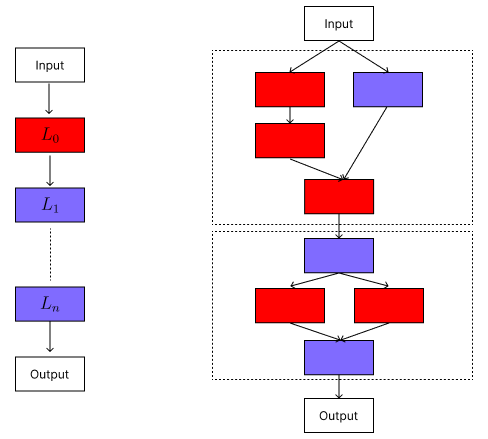
\includegraphics[width=8cm]{figures/cells.png}
    \caption{Left: chain-structured network, right: cells combined into an architecture}
    \label{fig:cells}
\end{figure}

\subsubsection{Directed Acyclic Graphs}
\Gls{DAG} is often used in \gls{NAS} to represent the structure of a neural network. In this context, the graph's vertices represent different operations or layers in the network, and the graph's edges represent the data flow between these operations. This allows researchers to efficiently represent and manipulate the structure of a neural network during the search process.

One of the main advantages of using \glspl{DAG} in \gls{NAS} is that they provide a convenient way to encode the constraints on the network architecture. For example, a \gls{DAG} can enforce the requirement that a neural network must have a certain number of layers or that individual layers must be connected in a specific way. This can help ensure that the search process only considers valid network architectures, which can speed up the search and improve its accuracy \autocite{https://doi.org/10.48550/arxiv.1806.09055}. 

In addition to representing the structure of a neural network, \glspl{DAG} can also represent the search space over which the architecture search algorithm operates. This allows the algorithm to explore different network architectures efficiently and evaluate their performance, ultimately discovering novel and effective network architectures \autocite{inproceedings}. 
